%%%%%%%%%%%%%%%%%%%%%%%%%%%%%%%%%%%%%%%%%%%%%%%%%%%%%%%%%%%%%%%%%%%%%%%%%%%%%%%%%%%%%%%%%%%%%%%
%%%%%%%%%%%%%%%%%%%%%%%%%%%%%%%%%%%%%%%%%%%%%%%%%%%%%%%%%%%%%%%%%%%%%%%%%%%%%%%%%%%%%%%%%%%%%%%
%% LaTeX-Beamer template for KIT design
%% by Erik Burger, Christian Hammer
%% title picture by Klaus Krogmann
%%
%% version 2.1
%%
%% mostly compatible to KIT corporate design v2.0
%% http://intranet.kit.edu/gestaltungsrichtlinien.php
%%
%% Problems, bugs and comments to
%% burger@kit.edu
%%
%%
%% Modified: 30.1.2013, Schwall

\documentclass[12pt]{beamer}

%% SLIDE FORMAT
\usepackage{templates/beamerthemekit}

%% german time format (e.g 30.1.2013)
\usepackage{datetime}
\usepackage{bbm} %% Used to denote the indicator function
%\usepackage[T1]{fontenc}
%\usepackage{amssymb}
\usepackage{amsmath}
\usepackage{graphicx}
\usepackage{color,psfrag}
\usepackage{subfig}

\newdateformat{germandate}{\THEDAY.\THEMONTH.\THEYEAR}
\newdateformat{americandate}{\THEMONTH/\THEDAY/\THEYEAR}

% use these packages for PCM symbols and UML classes
\usepackage{templates/tikzkit}
\usepackage{templates/tikzuml}
\usepackage{siunitx}

\usepackage{times}
\usepackage{tikz}


\usepackage[english]{babel}
\usepackage{csquotes}
\setquotestyle{american}
\usepackage[language=american,autocite=footnote,citestyle=authortitle,citetracker=true,backend=biber,babel=other]{biblatex}
\addbibresource{../refs.bib}

\usepackage{verbatim}
\usetikzlibrary{arrows,shapes}

\setbeamerfont{footnote}{size=\tiny}
%%%%%%%%%%%%%%%%%%%%%%%%%%%%%%%%%%%%%%%%%%%%%%%%%%%%%%%%%%%%%%%%%%%%%%%%%%%%%%%%%%%%%%%%%%%%%%%
%%%%%%%%%%%%%%%%%%%%%%%%%%%%%%%%%%%%%%%%%%%%%%%%%%%%%%%%%%%%%%%%%%%%%%%%%%%%%%%%%%%%%%%%%%%%%%%
% the presentation starts here

\usepackage{datetime}
\newdate{date}{11}{06}{2016}

% english vs. ngerman
\selectlanguage{english}

\title{\textbf{CRN\_IS9}: Performance Analysis of Hybrid Cognitive Radio
Systems with Imperfect Channel Knowledge
 }
\subtitle{ICC 2016, Kuala Lumpur, Malaysia}

\author{A. Kaushik\inst{1}, S.K. Sharma\inst{2}, S. Chatzinotas\inst{2}, B. Ottersten\inst{2}, F. K. Jondral\inst{1}}
\institute{\inst{1}Communications Engineering Lab, Karlsruhe Institute of Technology (KIT), Germany,\\
\and
\inst{2}SnT - securityandtrust.lu, University of Luxembourg, Luxembourg, \\
}

%% insert date in correct format
\iflanguage{english}{
	\date{11 June 2016}
	}{
	\date{\germandate\today}
}

\institute{\inst{1}CEL, Karlsruhe Institute of Technology (KIT), Germany and \inst{2}SnT, University of Luxembourg, Luxembourg}


%% Important macros and notations used in the dissertation are defined here

\newif\ifdebug
\debugfalse


\makeatletter
\if@twocolumn
	\newcommand{\figscalet}{0.71 \columnwidth}
	\newcommand{\figscalett}{\columnwidth}
	\newcommand{\figscale}{0.77 \columnwidth}
\else
	\newcommand{\figscale}{0.73\columnwidth}
	\newcommand{\figscalet}{0.7 \columnwidth}
	\newcommand{\figscalett}{\columnwidth}
\fi
\makeatother

% General Commands  
\newcommand{\e}[2]{{\mathbb E}_{#1}\left[ #2 \right]}    % Expectation
\newcommand{\s}[2]{{\frac{1}{{#1}}\sum_{n=1}^{#1}} {#2}}     % Summation 
\newcommand{\q}[2]{{\mathcal Q}_{#1}\left( #2 \right)}   % Macum Q function 
\newcommand{\p}{\mathbb P}				 % Probability
\newcommand{\sub}[1]{_{\text{#1}}}		         % Subscript as text
\newcommand{\supe}[1]{^{\text{#1}}}


% Probability 
\newcommand{\pd}{\text{P}\sub{d}}			 % Detection Probability 
\newcommand{\pfa}{\text{P}\sub{fa}}			 % False alarm Probability 
\newcommand{\pco}{\text{P}\sub{c}}			 % Confidence Probability 
\newcommand{\phz}{\p(\mathcal{H}_0)}                     % 0 Hypothesis  
\newcommand{\pho}{\p(\mathcal{H}_1)}			 % 1 Hypothesis  

%% Discrete Signals
\newcommand{\yrcvd}{y\sub{ST}}
\newcommand{\xp}{x\sub{PT}}
\newcommand{\xsfull}{x\sub{ST}}
\newcommand{\xscont}{x\sub{ST,cont}}
\newcommand{\ps}{P\sub{s}}
\newcommand{\ys}{y\sub{SR}}
\newcommand{\nap}{w}
\newcommand{\nas}{w}
\newcommand{\yp}{y\sub{PR}}
\newcommand{\xreg}{x\sub{ST,cont}}
\newcommand{\xtran}{x\sub{PR}}
\newcommand{\xtranpr}{x\sub{PR}}
\newcommand{\xtranst}{x\sub{ST}}
\newcommand{\xs}{x\sub{ST}}




% Signal to noise ratio
\newcommand{\snrp}{\frac{\ptranpt}{\npo}}
\newcommand{\snrs}{\frac{\ptranst}{\npo}}
\newcommand{\snrsi}{\frac{\npo}{\ptranst}}
\newcommand{\snrst}{\frac{\ps}{\sigma^2}}
\newcommand{\snrrcvd}{{\gamma}\sub{p,1}}
\newcommand{\snrso}{{\gamma}\sub{s}}
\newcommand{\snrpt}{{\gamma}\sub{p,2}}
\newcommand{\snrfull}{{\gamma}\sub{s, full}}
\newcommand{\snrcont}{{\gamma}\sub{s, cont}}
\newcommand{\snrsp}{\frac{|\ehs|^2 \ptranst}{\npo}\Big /\frac{\eprcvdsr}{\npo}}


% Distribution parameters 
\newcommand{\ls}{\lambda\sub{s}}
\newcommand{\Ks}{N\sub{s}}
\newcommand{\lp}{\lambda\sub{p}}
\newcommand{\Kp}{N\sub{p,2}}
\newcommand{\lpo}{\lambda\sub{p,1}}
\newcommand{\lpt}{\lambda\sub{p,2}}

\newcommand{\apo}{a\sub{p,1}}
\newcommand{\bpo}{b\sub{p,1}}
\newcommand{\apt}{a\sub{p,2}}
\newcommand{\bpt}{b\sub{p,2}}
\newcommand{\as}{a\sub{s}}
\newcommand{\bs}{b\sub{s}}
\newcommand{\ap}{a\sub{2}}
\newcommand{\bp}{b\sub{2}}

\newcommand{\mpo}{m\sub{p,1}}
\newcommand{\mpt}{m\sub{p,2}}
\newcommand{\ms}{m\sub{s}}
\newcommand{\acc}{\beta}


% Channel gain and power gain 
\newcommand{\hpo}{h\sub{p,1}}
\newcommand{\hptw}{h\sub{p,2}}
\newcommand{\hpth}{h\sub{p,3}}
\newcommand{\hs}{h\sub{s}}
\newcommand{\hpt}{h\sub{p,2}}

% Power
\newcommand{\ptran}{P\sub{Tx,PR}}
\newcommand{\preg}{P\sub{Tx,ST,cont}}
\newcommand{\pfull}{P\sub{Tx,ST,full}}
\newcommand{\npp}{\sigma^2\sub{w}}
\newcommand{\nps}{\sigma^2\sub{w}}
\newcommand{\npu}{\Delta\sigma^2}
\newcommand{\npo}{\sigma^2\sub{w}}
\newcommand{\spo}{\sigma^2\sub{s}}
\newcommand{\prcvdstpt}{P\sub{Rx,ST,$\hpo$}}
\newcommand{\prcvdsr}{P\sub{Rx,SR}}
\newcommand{\prcvdstpr}{P\sub{Rx,ST,$\hpth$}}
\newcommand{\ptranst}{P\sub{Tx,ST}}
\newcommand{\ptranpt}{P\sub{Tx,PT}}
\newcommand{\ptranpr}{P\sub{Tx,PR}}
\newcommand{\prcvdpr}{P\sub{Rx,PR}}
\newcommand{\prcvd}{P\sub{Rx,ST}}
\newcommand{\pp}{P\sub{p}}
\newcommand{\evar}{\frac{\npo}{2 \Ks}}


% Estimated parameters 
\newcommand{\eprcvdstpt}{\hat{P}\sub{Rx,ST,$\hpo$}}
\newcommand{\eprcvdstpr}{\hat{P}\sub{Rx,ST,$\hpth$}}
\newcommand{\eprcvdsr}{\hat{P}\sub{Rx,SR}}
\newcommand{\eprcvdpr}{\hat{P}\sub{Rx,PR}}
\newcommand{\epreg}{\hat{P}\sub{Tx,ST,cont}}
\newcommand{\ephs}{|\hat{h}\sub{s}|^2}
\newcommand{\ehpo}{\hat{h}\sub{p,1}}
\newcommand{\egpo}{\hat{h}\sub{p,1}}
\newcommand{\egpt}{\hat{h}\sub{p,2}}
\newcommand{\epgpo}{|\hat{h}\sub{p,1}|^2}
\newcommand{\epgpt}{|\hat{h}\sub{p,2}|^2}
\newcommand{\epgs}{|\hat{h}\sub{s}|^2}
\newcommand{\ehs}{\hat{h}\sub{s}}
\newcommand{\eprcvd}{\hat{P}\sub{Rx,ST}}
\newcommand{\ecz}{\hat{\text{C}}\sub{0}}
\newcommand{\eco}{\hat{\text{C}}\sub{1}}
\newcommand{\ectw}{\hat{\text{C}}\sub{2}}
\newcommand{\ecth}{\hat{\text{C}}\sub{3}}
\newcommand{\epd}{\hat{\text{P}}\sub{d}}
\newcommand{\eca}{\hat{\text{{C}}}\sub{s}}
\newcommand{\ers}{\hat{\text{{R}}}\sub{s}}
\newcommand{\ephpth}{|h\sub{p,3}|^2}

% Channels parameters
\newcommand{\phpo}{|h\sub{p,1}|^2}
\newcommand{\phptw}{|h\sub{p,2}|^2}
\newcommand{\phpth}{|h\sub{p,3}|^2}
\newcommand{\phs}{|h\sub{s}|^2}
\newcommand{\gpo}{h\sub{p,1}}
\newcommand{\gpt}{h\sub{p,2}}
\newcommand{\gs}{h\sub{s}}
\newcommand{\pgpo}{|h\sub{p,1}|^2}
\newcommand{\pgpt}{|h\sub{p,2}|^2}
\newcommand{\egs}{\hat{h}\sub{s}}
\newcommand{\pgs}{|h\sub{s}|^2}
\newcommand{\phpt}{|h\sub{p,2}|^2}


% System and performance paramters
\newcommand{\fsam}{f\sub{s}}
\newcommand{\flo}{f\sub{LOOfsset}}
\newcommand{\tsen}{\tau\sub{sen}}
\newcommand{\testpt}{\tau\sub{est, $\hpo$}}
\newcommand{\testptsr}{\tau\sub{est, $\hptw$}}
\newcommand{\testpr}{\tau\sub{est, $\hpth$}}
\newcommand{\ttestpt}{\tilde{\tau}\sub{est, $\hpo$}}
\newcommand{\ttestptsr}{\tilde{\tau}\sub{est, $\hptw$}}
\newcommand{\ttestpr}{\tilde{\tau}\sub{est, $\hpth$}}
\newcommand{\ttest}{\tilde{\tau}\sub{est}}
\newcommand{\ttsen}{\tilde{\tau}\sub{sen}}
\newcommand{\rs}{R\sub{s}}
\newcommand{\rsz}{R\sub{0}}
\newcommand{\rso}{R\sub{1}}
\newcommand{\rstw}{R\sub{2}}
\newcommand{\rsth}{R\sub{3}}
\newcommand{\trs}{R\sub{s}}
%\newcommand{\ers}{\e{}{\rs}}

\newcommand{\ca}{\text{C}\sub{s}}
\newcommand{\ttau}{\tilde{\tau}}

\newcommand{\test}{\tau\sub{est}}
\newcommand{\ttesto}{{\tau}^*\sub{est}}
\newcommand{\ttsenac}{\tilde{\tau}\sub{sen}\supe{}}
\newcommand{\ttsenoc}{\tilde{\tau}\sub{sen}\supe{}}

\newcommand{\rsac}{R\sub{s}\supe{AC}}
\newcommand{\rsoc}{R\sub{s}\supe{OC}}
\newcommand{\trsac}{{R}\sub{s}\supe{}}
\newcommand{\trsoc}{{R}\sub{s}\supe{}}


\newcommand{\cz}{\text{C}\sub{0}}
\newcommand{\co}{\text{C}\sub{1}}
\newcommand{\ctw}{\text{C}\sub{2}}
\newcommand{\cth}{\text{C}\sub{3}}

% Constraints and Thresholds
\newcommand{\ite}{\theta\sub{I}}     				% Interference Threshold
\newcommand{\opc}{\rho\sub{cont}}                               % Outage Probability Constraint on Controlled Power   
\newcommand{\opdc}{\rho\sub{d}}
\newcommand{\pdd}{\bar{\text{P}}\sub{d}}
\newcommand{\pcod}{\bar{\text{P}}\sub{c}}			 % Constraint on Confidence Probability 
\newcommand{\pc}{P\sub{Tx,ST,full}}
\newcommand{\mpd}{\rho\sub{d}}
\newcommand{\thric}{\mu\sub{IC}}
\newcommand{\thrac}{\mu\supe{}}
\newcommand{\throc}{\mu\supe{}}



% Distribution functions
\newcommand{\feprcvdstpt}{F_{\eprcvdstpt}}			% Estimated received power for the link ST - PT
\newcommand{\feprcvdstpr}{F_{\eprcvdstpr}}                      % Estimated received power for the link ST - PR 
\newcommand{\feprcvdsr}{F_{\eprcvdsr}}                          % Estimated received power for the link PT - SR 
\newcommand{\fprcvdpr}{F_{\eprcvdpr}}
\newcommand{\fephs}{F_{\ephs}}                                  % Estimated received power for the link ST - SR 
\newcommand{\fpd}{F_{\epd}}
\newcommand{\fcz}{F_{\ecz}}
\newcommand{\fco}{F_{\eco}}
\newcommand{\fctw}{F_{\ectw}}
\newcommand{\fcth}{F_{\ecth}}
\newcommand{\fprcvd}{F_{\eprcvd}}
\newcommand{\fgs}{F_{\epgs}}
\newcommand{\fgp}{F_{\epgpo}}
\newcommand{\fc}{F_{\ca}}
\newcommand{\fprcvdsr}{F_{\eprcvdsr}}
\newcommand{\fpreg}{F_{\epreg}}
\newcommand{\fpgpo}{F_{\pgpo}}
\newcommand{\fpgpt}{F_{\pgpt}}
\newcommand{\fpgs}{F_{\pgs}}
\newcommand{\feprcvd}{F_{\eprcvd}}
\newcommand{\fphpo}{F_{\phpo}}
\newcommand{\fphpt}{F_{\phpt}}
\newcommand{\fphs}{F_{\phs}}

% Density functions
\newcommand{\dprcvdstpt}{f_{\prcvdstpt}}
\newcommand{\dpreg}{f_{\epreg}}
\newcommand{\dhs}{f_{\hs}}
\newcommand{\drs}{f_{\ers}}
\newcommand{\dcz}{f_{\ecz}}
\newcommand{\dco}{f_{\eco}}
\newcommand{\dctw}{f_{\ectw}}
\newcommand{\dcth}{f_{\ecth}}
\newcommand{\dpd}{f_{\epd}}
\newcommand{\dc}{f_{\ca}}
\newcommand{\dsnrs}{f_{\frac{ |\ehs|^2 \ptranst}{\npo}}}
\newcommand{\dsnrp}{f_{\frac{\eprcvdsr}{\npo}}}
\newcommand{\dsnrsp}{f_{\frac{|\ehs|^2 \ptranst}{\npo}\Big /\frac{\eprcvdsr}{\npo}}}
\newcommand{\dprcvd}{f_{\eprcvd}}
\newcommand{\dprcvdpr}{f_{\eprcvdpr}}


\newcommand{\imp}{\uline}
\newcommand{\ur}{\uuline}
\newcommand{\ns}{\uwave} 
\newcommand{\ws}{\sout}
\newcommand{\fl}{\dashuline}
\newcommand{\un}{\dotuline}

% Define new mathmatical operators 
\DeclareMathOperator*{\maxi}{max}
\DeclareMathOperator*{\gthan}{\ge}
\DeclareMathOperator*{\eqto}{=}
\DeclareMathOperator*{\cchi2}{\mathcal{X}^2}
\DeclareMathOperator*{\ncchi2}{\mathcal{X}_1^2}
\DeclareMathOperator*{\ts}{\text{T}(\textbf{y})}
\DeclareMathOperator*{\argmaxi}{argmax}


% Theorem Stuff
\newtheorem{theorem}{Theorem}
\newtheorem{case}{Case}
\newtheorem{constraint}{Constraint}
\newtheorem{lemma}{Lemma}
\newtheorem{prop}{Proposition}
\newtheorem{remark}{Remark}
\newtheorem{coro}{Corollary}
\newtheorem{defi}{Definition}
\newtheorem{approxi}{Approximation}

% derrived Expressions
\newcommand{\lambdas}{\frac{\sigma_w^4}{ 2 \Ks \ptranst}}
\newcommand{\lambdasinv}{\frac{2 \Ks \ptranst}{\sigma_w^4}}



\newcommand{\fs}[2]{\fontsize{#1 pt}{#2}\selectfont}


\hyphenation{under-estimation over-estimation}

% Position the text inside the frame
\usepackage[absolute,overlay]{textpos}

\addtobeamertemplate{footnote}{}{\vspace{1.0ex}}
\addtolength{\footnotesep}{-5mm} % change to 1mm

\begin{document}

\newcommand\FrameText[1]{%
  \begin{textblock*}{\paperwidth}(0pt,\textheight)
    \raggedright #1\hspace{.5em}
  \end{textblock*}}



%title page
\begin{frame}
	\titlepage
\end{frame}

%%%%%%%%%%%%%%%%%%%%%%%%%%%%%%%%%%%%%%%%%%%%%%%%%%%% Frame %%%%%%%%%%%%%%%%%%%%%%%%%%%%%%%%%%%%%%%%%%%%%%%%%%%%%%       
\begin{frame}{Contents}
        \fs{10}{15}
        \begin{itemize}
                \item Hybrid Scenario 
                \item Signal Model
                \item Problem Description 
                \item Proposed Approach 
                \item Numerical Analysis
                \item Summary
        \end{itemize}
\end{frame}


%%%%%%%%%%%%%%%%%%%%%%%%%%%%%%%%%%%%%%%%%%%%%%%%%%%% Frame %%%%%%%%%%%%%%%%%%%%%%%%%%%%%%%%%%%%%%%%%%%%%%%%%%%%%%       
\begin{frame}[t]{Hybrid Scenario}
        \begin{overlayarea}{\textwidth}{4.4cm}
        \begin{center}
                \only<1->
                {
                        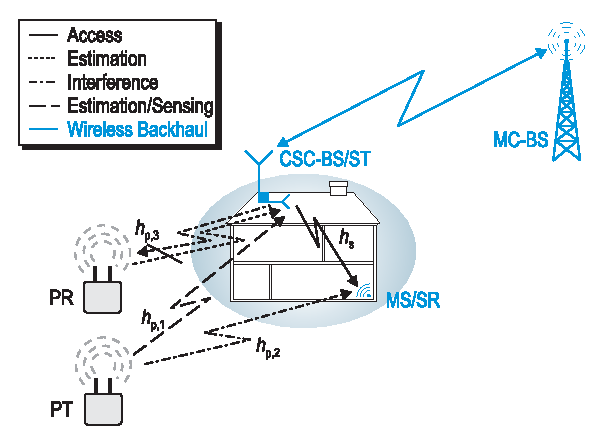
\includegraphics[width = 0.45 \paperwidth]{../figures/CR_Scenario_Hybrid}
                }
        \end{center}
        \end{overlayarea}
        \only<1>{
                \fs{8}{8}
                Hybrid System:
                \begin{itemize}
                        \item A spectrum sensing and a power control mechanism is employed at the ST
                        \item To accomplish this $\Rightarrow$ Knowledge of the channels $\hpo, \hpth$ is required at ST
			\item Further, to characterize the throughput at SR $\Rightarrow$ Knowledge of the channels $\hptw, \hs$ is required at ST
                \end{itemize}
                In a realistic scenario:
                \begin{itemize}
                \item Channel knowledge is not available at the ST, \keyword{Solution} needs to be estimated
                \item Without any knowledge of the primary system, direct estimation of channel is not possible
                \end{itemize}
        }
        \only<2->{
                \fs{8}{8}
                Contributions:
                \begin{itemize}
                        \item We propose an analytical framework that facilitates a successful incorporation of the estimation of the involved channels 
                        \item We examine the impact of channel knowledge in terms of interference encountered  
                        \item We depict a estimation-sensing-throughput tradeoff that allow us to optimize the performance of the hybrid system
                \end{itemize}
        }
\end{frame}


%%%%%%%%%%%%%%%%%%%%%%%%%%%%%%%%%%%%%%%%%%%%%%%%%%%%% Frame %%%%%%%%%%%%%%%%%%%%%%%%%%%%%%%%%%%%%%%%%%%%%%%%%%%%%%       
%\begin{frame}{Assumptions and Considerations}
%        \begin{columns}
%                \begin{column}{0.5 \paperwidth}
%                        \begin{center}
%                                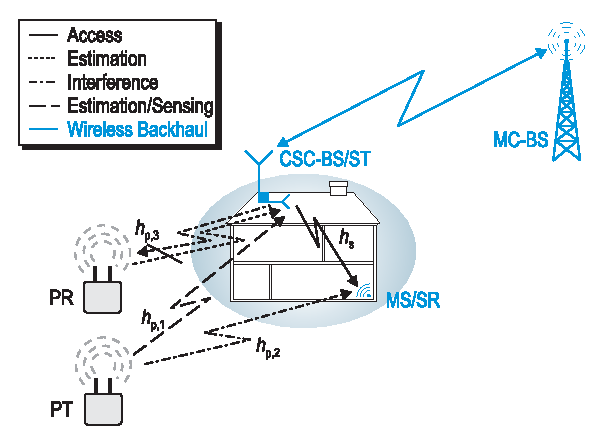
\includegraphics[width = 0.38 \paperwidth]{../figures/CR_Scenario_Hybrid}
%                        \end{center}
%                \end{column}
%                \begin{column}{0.5 \paperwidth}
%                        \begin{center}
%                                \includegraphics[width = 0.42 \paperwidth]{../figures/Frame_Structure}
%                        \end{center}
%                \end{column}
%        \end{columns}
%        \vspace{0.5cm}
%        \begin{itemize}
%                \fs{8}{10}
%                \item Coherence time of the channel $\approx T$
%                \item Power control at the ST is done by listening to the beacon or neighbouring pilot channel sent by the PR $\implies$ Channel reciprocity
%                \item In each frame, the ST performs estimation of the received power followed by data transmission with controlled power
%                \item In listening mode, ST considers proper alignment of the PR transmissions $\implies$ no interference is encountered at the SR from the PR
%                \item Transmit power of the PR is known at the ST
%        \end{itemize}
%
%\end{frame}

%%%%%%%%%%%%%%%%%%%%%%%%%%%%%%%%%%%%%%%%%%%%%%%%%%%% Frame %%%%%%%%%%%%%%%%%%%%%%%%%%%%%%%%%%%%%%%%%%%%%%%%%%%%%%       
\begin{frame}{Signal Model}
        %\vspace{-0.5cm}
        \fs{8}{8}
        \begin{columns}[t]
                \begin{column}{0.51 \paperwidth}
                \vspace{-0.4cm}
                \begin{itemize}
                     \item Received signal at the ST
                        \begin{equation*}
			\yrcvd[n] = 
				\begin{cases}
				\hpo \cdot \xp[n] + w[n] & : \mathcal{H}_1 \\
				w[n] & :\mathcal{H}_0
				\end{cases}
                        \end{equation*}
                     \item Received signal at the PR
                        \begin{equation*}
                        \yp[n] = 
			\begin{cases}
			\hpth \cdot \xscont[n] + w[n] & : \pd \\
			\hpth \cdot \xsfull[n] + w[n] & : 1- \pd 
			\end{cases}
			\end{equation*}
                     \item Received signal at the SR
                        \begin{equation*}
                                \ys[n] = 
				\begin{cases}
					\hs \cdot \xsfull[n] + \hptw \cdot \xp[n] + w[n] &: 1 - \pd \\
					\hs \cdot \xsfull[n] + w[n] &: 1 - \pfa \\
					\hs \cdot \xscont[n] + \hptw \cdot \xp[n] + w[n] &: \pd \\
					\hs \cdot \xscont[n] + w[n] &: \pfa 
					\end{cases}
                        \end{equation*}
                \end{itemize}
                \end{column}
                \begin{column}{0.06 \paperwidth}
                \end{column}
                \begin{column}{0.43 \paperwidth}
                \begin{center}
                        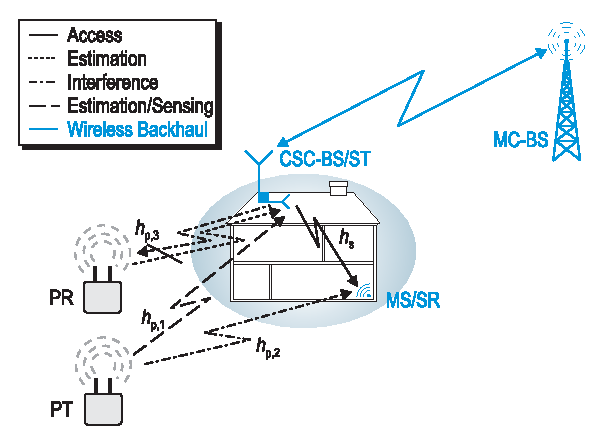
\includegraphics[width = 0.38 \paperwidth]{../figures/CR_Scenario_Hybrid}
                \end{center}
                \end{column}
        \end{columns}
\end{frame}

%%%%%%%%%%%%%%%%%%%%%%%%%%%%%%%%%%%%%%%%%%%%%%%%%%%% Frame %%%%%%%%%%%%%%%%%%%%%%%%%%%%%%%%%%%%%%%%%%%%%%%%%%%%%%       
\begin{frame}{Problem Description}
        %\vspace{-0.5cm}
        \fs{8}{8}
		\begin{itemize}
		\item Existing models (Ideal Model)
		\end{itemize}
		\vspace{-0.2cm}
                     \begin{align*}
	             	\text{Interference constraint} 
			\begin{cases}
			\pho \cdot \pd \cdot \phpth \preg \le \ite \\
		     	\text{and   } \pho \cdot (1 - \pd) \cdot \phpth \pfull \le \ite			    	\end{cases} 
		     \end{align*}
		\vspace{-0.2cm}
                     \begin{align*}
		        \text{Throughput at SR}
			\begin{cases}		
			\rsz(\tsen) =& \frac{T- \tsen}{T} \cdot \log_2 \left(1 + |\hs|^2 \frac{\pfull}{\npo}\right) (1 - \pfa ) \cdot \phz,  \\ 
			\rso(\tsen) =& \frac{T- \tsen}{T} \log_2 \left(1 + \frac{|\hs|^2 \pfull }{|\hptw|^2 \ptranpt  + \npo} \right) (1 - \pd) \cdot \pho,  \\ 
			\rstw(\tsen) =& \frac{T- \tsen}{T} \cdot \log_2 \left(1 + |\hs|^2 \frac{\preg}{\npo}\right) \pfa \cdot \phz,  \\ 
			\rsth(\tsen) =& \frac{T- \tsen}{T} \cdot \log_2 \left(1 + \frac{|\hs|^2 \preg }{|\hptw|^2 \ptranpt  + \npo} \right) \pd \cdot \pho.  
			\end{cases}
		     \end{align*}
                \begin{itemize}
                \item Without the knowledge of received power (sensing channel, $\hpo$), the characterization of $\pd$ at the ST is not possible
		\item Without the knowledge of the interference channel towards the PR ($\hpth$), the power control mechanism cannot be employed at the ST
		\item The knowledge of the access ($\hs$) and the interference channel ($\hptw$) to the SR, from the PT, is required at the ST for characterizing the SU throughput.
		\end{itemize}
\end{frame}

%%%%%%%%%%%%%%%%%%%%%%%%%%%%%%%%%%%%%%%%%%%%%%%%%%%% Frame %%%%%%%%%%%%%%%%%%%%%%%%%%%%%%%%%%%%%%%%%%%%%%%%%%%%%%       
\begin{frame}{Proposed Approach}
        \begin{overlayarea}{\textwidth}{4.4cm}
        \begin{center}
		\fs{8}{8}
		Proposed frame structure for the secondary system \\
        	\vspace{0.4cm}
                \includegraphics[width = 0.45 \paperwidth]{../figures/Frame_Structure}
	\end{center}
	\end{overlayarea}
	\fs{8}{8}
	\begin{itemize}
	\item We consider the estimation of involved channels. In order to facilitate deployment received power estimation is proposed for the sensing and interference channel. 
	\item Next, we characterize the variations due to channel estimation in the estimation parameters in terms of their pdfs.
	\item We further characterize the aforementioned variations, which include the interference received at PR and expected throughput at SR in terms of their cdf.
	\item We utilize these cdfs to obtain the expression estimation-sensing-throughput tradeoff. 
	\end{itemize}	
\end{frame}

%%%%%%%%%%%%%%%%%%%%%%%%%%%%%%%%%%%%%%%%%%%%%%%%%%%% Frame %%%%%%%%%%%%%%%%%%%%%%%%%%%%%%%%%%%%%%%%%%%%%%%%%%%%%%       
\begin{frame}{Performance Characterization}
        \vspace{-0.8cm}
        \fs{8}{8}
		\begin{columns}[t]
                \begin{column}{0.52 \paperwidth}
		\begin{center}	%\begin{itemize}
			%\item 
			\textbf{Channel Estimation} 
			\begin{itemize}
       		 	\fs{8}{8}
                	     \item Sensing channel
            		\vspace{-0.2cm}     
			\begin{align*}
			    	 \feprcvdstpt(x) = 1 - \Gamma \left( \frac{\testpt \fsam}{2}, \frac{\testpt \fsam x}{2 \prcvdstpt} \right) 
		     	     \end{align*}
		     	\item Access channel	
            		\vspace{-0.2cm}     
                     	\begin{align*}
		   		\fephs(x) \approx 1 - \Gamma \left(a, \frac{x}{b} \right)   
		     	\end{align*}
		     	\item Interference channel	
            		\vspace{-0.2cm}     
                     	\begin{align*}
		   		\feprcvdsr(x) = 1 - \Gamma \left( \frac{\testptsr \fsam}{2}, \frac{\testptsr \fsam x}{2 \prcvdsr} \right) 
		     	\end{align*}
		     	\item Interference channel	
            		\vspace{-0.2cm}     
                     	\begin{align*}
		     		\feprcvdstpr(x) = 1 - \Gamma \left( \frac{\testpr \fsam}{2}, \frac{\testpr \fsam x}{2 \prcvdstpr} \right)
			\end{align*}
		\end{itemize}
	\end{center}		
	%\end{itemize}
	\end{column}
        \begin{column}{0.48 \paperwidth}
		\begin{center}		
		\textbf{Detection probability constraint} 
		\begin{align*}
		\p(\pd(\eprcvdstpt) \le \pdd) &\le \opdc \\
		\end{align*}
		\textbf{Interference constraint} 
		\begin{align*}
		\p(\prcvdpr(\pd(\eprcvdstpt), \eprcvdstpr) \ge \ite) &\le \opc 
		\end{align*}
		\textbf{Expected secondary throughput}
		\begin{align*}
		\e{\Omega}{\rs(\tsen)} &= \frac{T - \testpr - \tsen}{T} \cdot \\ &\Bigg[ (1 - \pfa) \cdot \phz \cdot \e{\cz}{\cz} + \\  & (1 - \e{\pd}\pd) \cdot \pho \cdot \e{\co}{\co}  + \\ &\pfa \cdot \phz \cdot \e{\ctw}{\ctw} +  \nonumber \\ & \e{\pd}{\pd} \cdot \pho \cdot \e{\cth}{\cth} \Bigg]. 
		\end{align*}
		\end{center}
	\end{column}
	\end{columns}
\end{frame}


%%%%%%%%%%%%%%%%%%%%%%%%%%%%%%%%%%%%%%%%%%%%%%%%%%%% Frame %%%%%%%%%%%%%%%%%%%%%%%%%%%%%%%%%%%%%%%%%%%%%%%%%%%%%%       
\begin{frame}{Performance Characterization}
        \fs{8}{8}
		\begin{center}	
		\begin{itemize}
		\item \keyword{Theorem}: The expected achievable SU throughput subject to an outage constraint on detection probability at the ST and an outage constraint on interference power at the PR given by
		\begin{align*}
		\rs(\ttsen) &= \maxi_{\tsen, \preg} \e{\Omega}{\rs(\tsen)} \\
		\text{s.t.} & \text{ }\; \p(\pd \le \pdd) \le \opdc \\
		\text{s.t.} & \text{ }\; \p(\prcvdpr \ge \ite) \le \opc 
		\end{align*}
		\end{itemize}
		\end{center}
\end{frame}


%%%%%%%%%%%%%%%%%%%%%%%%%%%%%%%%%%%%%%%%%%%%%%%%%%%%% Frame %%%%%%%%%%%%%%%%%%%%%%%%%%%%%%%%%%%%%%%%%%%%%%%%%%%%%%
\begin{frame}{Numerical Analysis}
\fs{8}{8}
\begin{center}
\renewcommand{\arraystretch}{1.3}
\begin{tabular}{c||c|c}
\hline
\bfseries Parameter & \bfseries Definition & \bfseries Value \\
\hline\hline
$\fsam$ & Sampling Frequency & $\SI{1}{MHz}$ \\
$T$ & Frame Duration & $\SI{100}{ms}$ \\
$\testpt$ & Estimation time for the channel $\hpo$ & $\SI{1}{ms}$ \\
$\testptsr$ & Estimation time for the channel $\hptw$ & $\SI{1}{ms}$ \\
$\testpr$ & Estimation time for the channel $\hpth$ & $\SI{1}{ms}$ \\
$\phpo$ & Power gain for channel $\hpo$ & $\SI{-120}{dB}$ \\
$\phptw$ & Power gain for channel $\hptw$ & $\SI{-120}{dB}$ \\
$\phpth$ & Power gain for channel $\hpth$ &$\SI{-100}{dB}$ \\
$\phs$ & Power gain for channel $\hs$ &$\SI{-80}{dB}$ \\
$\ite$ & Interference threshold &$\SI{-110}{dBm}$ \\
$\opc$ & Outage constraint on interference power at PR& $0.1$ \\
$\opdc$ & Outage constraint on detection probability & $0.1$ \\
$\nps$ & Transmit power at PT and PR&$\SI{10}{dBm}$ \\
$\npo$ & Noise power at ST, SR and PR &$\SI{-100}{dBm}$ \\
$\pdd$ & Detection probability threshold  &$0.9$ \\
$\phz$ & Occurrence Probability for hypothesis $\mathcal H_0$ & $0.2$ \\
$\pfull$ & Transmit power at ST &$\SI{0}{dBm}$ \\
$\Ks$ & Number of pilot symbols & 10 \\ \hline
\end{tabular}
\end{center}
\end{frame}

%%%%%%%%%%%%%%%%%%%%%%%%%%%%%%%%%%%%%%%%%%%%%%%%%%%%% Frame %%%%%%%%%%%%%%%%%%%%%%%%%%%%%%%%%%%%%%%%%%%%%%%%%%%%%%
\begin{frame}{Numerical Analysis}
        \begin{overlayarea}{\textwidth}{6.0cm}
        \begin{center}
                \fs{8}{8}
                Sensing-throughput tradeoff for $\testpt = \testptsr =  \testpr = \SI{1}{ms}$ \\ 
                % This file is generated by the MATLAB m-file laprint.m. It can be included
% into LaTeX documents using the packages graphicx, color and psfrag.
% It is accompanied by a postscript file. A sample LaTeX file is:
%    \documentclass{article}\usepackage{graphicx,color,psfrag}
%    \begin{document}% This file is generated by the MATLAB m-file laprint.m. It can be included
% into LaTeX documents using the packages graphicx, color and psfrag.
% It is accompanied by a postscript file. A sample LaTeX file is:
%    \documentclass{article}\usepackage{graphicx,color,psfrag}
%    \begin{document}% This file is generated by the MATLAB m-file laprint.m. It can be included
% into LaTeX documents using the packages graphicx, color and psfrag.
% It is accompanied by a postscript file. A sample LaTeX file is:
%    \documentclass{article}\usepackage{graphicx,color,psfrag}
%    \begin{document}\input{fig_thr_sen_time_tradeoff_AWGN}\end{document}
% See http://www.mathworks.de/matlabcentral/fileexchange/loadFile.do?objectId=4638
% for recent versions of laprint.m.
%
% created by:           LaPrint version 3.16 (13.9.2004)
% created on:           12-Jul-2016 14:47:00
% eps bounding box:     16 cm x 12 cm
% comment:              
%
%\begin{psfrags}%
%\psfragscanon%
%
% text strings:
\psfrag{s08}[b][b]{\fontsize{8}{12}\fontseries{m}\mathversion{normal}\fontshape{n}\selectfont \color[rgb]{0,0,0}\setlength{\tabcolsep}{0pt}\begin{tabular}{c}$\rs(\test = \SI{5}{ms}, \tsen)$ [bits/sec/Hz]\end{tabular}}%
\psfrag{s09}[t][t]{\fontsize{8}{12}\fontseries{m}\mathversion{normal}\fontshape{n}\selectfont \color[rgb]{0,0,0}\setlength{\tabcolsep}{0pt}\begin{tabular}{c}$\tsen$ [ms]\end{tabular}}%
\psfrag{s13}[][]{\fontsize{10}{15}\fontseries{m}\mathversion{normal}\fontshape{n}\selectfont \color[rgb]{0,0,0}\setlength{\tabcolsep}{0pt}\begin{tabular}{c} \end{tabular}}%
\psfrag{s14}[][]{\fontsize{10}{15}\fontseries{m}\mathversion{normal}\fontshape{n}\selectfont \color[rgb]{0,0,0}\setlength{\tabcolsep}{0pt}\begin{tabular}{c} \end{tabular}}%
\psfrag{s15}[l][l]{\fontsize{8}{12}\fontseries{m}\mathversion{normal}\fontshape{n}\selectfont \color[rgb]{0,0,0}Simulated}%
\psfrag{s16}[l][l]{\fontsize{8}{12}\fontseries{m}\mathversion{normal}\fontshape{n}\selectfont \color[rgb]{0,0,0}IM}%
\psfrag{s17}[l][l]{\fontsize{8}{12}\fontseries{m}\mathversion{normal}\fontshape{n}\selectfont \color[rgb]{0,0,0}EM-AC, Problem 1}%
\psfrag{s18}[l][l]{\fontsize{8}{12}\fontseries{m}\mathversion{normal}\fontshape{n}\selectfont \color[rgb]{0,0,0}EM-OC, Problem 2}%
\psfrag{s19}[l][l]{\fontsize{8}{12}\fontseries{m}\mathversion{normal}\fontshape{n}\selectfont \color[rgb]{0,0,0}$\trs(\test,\ttsen)$}%
\psfrag{s20}[l][l]{\fontsize{8}{12}\fontseries{m}\mathversion{normal}\fontshape{n}\selectfont \color[rgb]{0,0,0}Simulated}%
\psfrag{s21}[b][b]{\fontsize{8}{12}\fontseries{m}\mathversion{normal}\fontshape{n}\selectfont \color[rgb]{0,0,0}\setlength{\tabcolsep}{0pt}\begin{tabular}{c}Zoom\end{tabular}}%
%
% axes font properties:
\fontsize{8}{12}\fontseries{m}\mathversion{normal}%
\fontshape{n}\selectfont%
%
% xticklabels:
\psfrag{x01}[t][t]{5}%
\psfrag{x02}[t][t]{5.2}%
\psfrag{x03}[t][t]{5.4}%
\psfrag{x04}[t][t]{5.6}%
\psfrag{x05}[t][t]{1}%
\psfrag{x06}[t][t]{2}%
\psfrag{x07}[t][t]{3}%
\psfrag{x08}[t][t]{4}%
\psfrag{x09}[t][t]{5}%
\psfrag{x10}[t][t]{6}%
\psfrag{x11}[t][t]{7}%
\psfrag{x12}[t][t]{8}%
\psfrag{x13}[t][t]{9}%
\psfrag{x14}[t][t]{10}%
%
% yticklabels:
\psfrag{v01}[r][r]{2.55}%
\psfrag{v02}[r][r]{2.6}%
\psfrag{v03}[r][r]{2.65}%
\psfrag{v04}[r][r]{0}%
\psfrag{v05}[r][r]{0.5}%
\psfrag{v06}[r][r]{1}%
\psfrag{v07}[r][r]{1.5}%
\psfrag{v08}[r][r]{2}%
\psfrag{v09}[r][r]{2.5}%
%
% Figure:
%\resizebox{8cm}{!}{\includegraphics{fig_thr_sen_time_tradeoff_AWGN.eps}}%
%\end{psfrags}%
%
% End fig_thr_sen_time_tradeoff_AWGN.tex
\end{document}
% See http://www.mathworks.de/matlabcentral/fileexchange/loadFile.do?objectId=4638
% for recent versions of laprint.m.
%
% created by:           LaPrint version 3.16 (13.9.2004)
% created on:           12-Jul-2016 14:47:00
% eps bounding box:     16 cm x 12 cm
% comment:              
%
%\begin{psfrags}%
%\psfragscanon%
%
% text strings:
\psfrag{s08}[b][b]{\fontsize{8}{12}\fontseries{m}\mathversion{normal}\fontshape{n}\selectfont \color[rgb]{0,0,0}\setlength{\tabcolsep}{0pt}\begin{tabular}{c}$\rs(\test = \SI{5}{ms}, \tsen)$ [bits/sec/Hz]\end{tabular}}%
\psfrag{s09}[t][t]{\fontsize{8}{12}\fontseries{m}\mathversion{normal}\fontshape{n}\selectfont \color[rgb]{0,0,0}\setlength{\tabcolsep}{0pt}\begin{tabular}{c}$\tsen$ [ms]\end{tabular}}%
\psfrag{s13}[][]{\fontsize{10}{15}\fontseries{m}\mathversion{normal}\fontshape{n}\selectfont \color[rgb]{0,0,0}\setlength{\tabcolsep}{0pt}\begin{tabular}{c} \end{tabular}}%
\psfrag{s14}[][]{\fontsize{10}{15}\fontseries{m}\mathversion{normal}\fontshape{n}\selectfont \color[rgb]{0,0,0}\setlength{\tabcolsep}{0pt}\begin{tabular}{c} \end{tabular}}%
\psfrag{s15}[l][l]{\fontsize{8}{12}\fontseries{m}\mathversion{normal}\fontshape{n}\selectfont \color[rgb]{0,0,0}Simulated}%
\psfrag{s16}[l][l]{\fontsize{8}{12}\fontseries{m}\mathversion{normal}\fontshape{n}\selectfont \color[rgb]{0,0,0}IM}%
\psfrag{s17}[l][l]{\fontsize{8}{12}\fontseries{m}\mathversion{normal}\fontshape{n}\selectfont \color[rgb]{0,0,0}EM-AC, Problem 1}%
\psfrag{s18}[l][l]{\fontsize{8}{12}\fontseries{m}\mathversion{normal}\fontshape{n}\selectfont \color[rgb]{0,0,0}EM-OC, Problem 2}%
\psfrag{s19}[l][l]{\fontsize{8}{12}\fontseries{m}\mathversion{normal}\fontshape{n}\selectfont \color[rgb]{0,0,0}$\trs(\test,\ttsen)$}%
\psfrag{s20}[l][l]{\fontsize{8}{12}\fontseries{m}\mathversion{normal}\fontshape{n}\selectfont \color[rgb]{0,0,0}Simulated}%
\psfrag{s21}[b][b]{\fontsize{8}{12}\fontseries{m}\mathversion{normal}\fontshape{n}\selectfont \color[rgb]{0,0,0}\setlength{\tabcolsep}{0pt}\begin{tabular}{c}Zoom\end{tabular}}%
%
% axes font properties:
\fontsize{8}{12}\fontseries{m}\mathversion{normal}%
\fontshape{n}\selectfont%
%
% xticklabels:
\psfrag{x01}[t][t]{5}%
\psfrag{x02}[t][t]{5.2}%
\psfrag{x03}[t][t]{5.4}%
\psfrag{x04}[t][t]{5.6}%
\psfrag{x05}[t][t]{1}%
\psfrag{x06}[t][t]{2}%
\psfrag{x07}[t][t]{3}%
\psfrag{x08}[t][t]{4}%
\psfrag{x09}[t][t]{5}%
\psfrag{x10}[t][t]{6}%
\psfrag{x11}[t][t]{7}%
\psfrag{x12}[t][t]{8}%
\psfrag{x13}[t][t]{9}%
\psfrag{x14}[t][t]{10}%
%
% yticklabels:
\psfrag{v01}[r][r]{2.55}%
\psfrag{v02}[r][r]{2.6}%
\psfrag{v03}[r][r]{2.65}%
\psfrag{v04}[r][r]{0}%
\psfrag{v05}[r][r]{0.5}%
\psfrag{v06}[r][r]{1}%
\psfrag{v07}[r][r]{1.5}%
\psfrag{v08}[r][r]{2}%
\psfrag{v09}[r][r]{2.5}%
%
% Figure:
%\resizebox{8cm}{!}{\includegraphics{fig_thr_sen_time_tradeoff_AWGN.eps}}%
%\end{psfrags}%
%
% End fig_thr_sen_time_tradeoff_AWGN.tex
\end{document}
% See http://www.mathworks.de/matlabcentral/fileexchange/loadFile.do?objectId=4638
% for recent versions of laprint.m.
%
% created by:           LaPrint version 3.16 (13.9.2004)
% created on:           12-Jul-2016 14:47:00
% eps bounding box:     16 cm x 12 cm
% comment:              
%
%\begin{psfrags}%
%\psfragscanon%
%
% text strings:
\psfrag{s08}[b][b]{\fontsize{8}{12}\fontseries{m}\mathversion{normal}\fontshape{n}\selectfont \color[rgb]{0,0,0}\setlength{\tabcolsep}{0pt}\begin{tabular}{c}$\rs(\test = \SI{5}{ms}, \tsen)$ [bits/sec/Hz]\end{tabular}}%
\psfrag{s09}[t][t]{\fontsize{8}{12}\fontseries{m}\mathversion{normal}\fontshape{n}\selectfont \color[rgb]{0,0,0}\setlength{\tabcolsep}{0pt}\begin{tabular}{c}$\tsen$ [ms]\end{tabular}}%
\psfrag{s13}[][]{\fontsize{10}{15}\fontseries{m}\mathversion{normal}\fontshape{n}\selectfont \color[rgb]{0,0,0}\setlength{\tabcolsep}{0pt}\begin{tabular}{c} \end{tabular}}%
\psfrag{s14}[][]{\fontsize{10}{15}\fontseries{m}\mathversion{normal}\fontshape{n}\selectfont \color[rgb]{0,0,0}\setlength{\tabcolsep}{0pt}\begin{tabular}{c} \end{tabular}}%
\psfrag{s15}[l][l]{\fontsize{8}{12}\fontseries{m}\mathversion{normal}\fontshape{n}\selectfont \color[rgb]{0,0,0}Simulated}%
\psfrag{s16}[l][l]{\fontsize{8}{12}\fontseries{m}\mathversion{normal}\fontshape{n}\selectfont \color[rgb]{0,0,0}IM}%
\psfrag{s17}[l][l]{\fontsize{8}{12}\fontseries{m}\mathversion{normal}\fontshape{n}\selectfont \color[rgb]{0,0,0}EM-AC, Problem 1}%
\psfrag{s18}[l][l]{\fontsize{8}{12}\fontseries{m}\mathversion{normal}\fontshape{n}\selectfont \color[rgb]{0,0,0}EM-OC, Problem 2}%
\psfrag{s19}[l][l]{\fontsize{8}{12}\fontseries{m}\mathversion{normal}\fontshape{n}\selectfont \color[rgb]{0,0,0}$\trs(\test,\ttsen)$}%
\psfrag{s20}[l][l]{\fontsize{8}{12}\fontseries{m}\mathversion{normal}\fontshape{n}\selectfont \color[rgb]{0,0,0}Simulated}%
\psfrag{s21}[b][b]{\fontsize{8}{12}\fontseries{m}\mathversion{normal}\fontshape{n}\selectfont \color[rgb]{0,0,0}\setlength{\tabcolsep}{0pt}\begin{tabular}{c}Zoom\end{tabular}}%
%
% axes font properties:
\fontsize{8}{12}\fontseries{m}\mathversion{normal}%
\fontshape{n}\selectfont%
%
% xticklabels:
\psfrag{x01}[t][t]{5}%
\psfrag{x02}[t][t]{5.2}%
\psfrag{x03}[t][t]{5.4}%
\psfrag{x04}[t][t]{5.6}%
\psfrag{x05}[t][t]{1}%
\psfrag{x06}[t][t]{2}%
\psfrag{x07}[t][t]{3}%
\psfrag{x08}[t][t]{4}%
\psfrag{x09}[t][t]{5}%
\psfrag{x10}[t][t]{6}%
\psfrag{x11}[t][t]{7}%
\psfrag{x12}[t][t]{8}%
\psfrag{x13}[t][t]{9}%
\psfrag{x14}[t][t]{10}%
%
% yticklabels:
\psfrag{v01}[r][r]{2.55}%
\psfrag{v02}[r][r]{2.6}%
\psfrag{v03}[r][r]{2.65}%
\psfrag{v04}[r][r]{0}%
\psfrag{v05}[r][r]{0.5}%
\psfrag{v06}[r][r]{1}%
\psfrag{v07}[r][r]{1.5}%
\psfrag{v08}[r][r]{2}%
\psfrag{v09}[r][r]{2.5}%
%
% Figure:
%\resizebox{8cm}{!}{\includegraphics{fig_thr_sen_time_tradeoff_AWGN.eps}}%
%\end{psfrags}%
%
% End fig_thr_sen_time_tradeoff_AWGN.tex

		\centering
		\begin{tikzpicture}[scale=1]
		\node[anchor=south west,inner sep=0] (image) at (0,0)
		{
       			\includegraphics[width= \figscale]{../figures/fig_thr_sen_time_tradeoff_AWGN}
		};
		\begin{scope}[x={(image.south east)},y={(image.north west)}]

		\draw[black,thick,<->] (0.105,0.13) --  node[above, font=\scriptsize] {$\testpt = \testptsr = \testpr$} (0.16,0.13);

		\draw[black,->] (0.23,0.53) -- (0.18,0.65);
		\node[draw=none,font=\scriptsize] at (0.32,0.48) {$\opdc \in \{0.05,0.10\}$};
                %\draw[help lines,xstep=.1,ystep=.1] (0,0) grid (1,1);
                %\foreach \x in {0,1,...,9} { \node [anchor=north] at (\x/10,0) {0.\x}; }
                %\foreach \y in {0,1,...,9} { \node [anchor=east] at (0,\y/10) {0.\y}; }
                \end{scope}
                \end{tikzpicture}
        \end{center}
        \end{overlayarea}
        \fs{8}{8}
        \begin{itemize}
                \item As indicated by the margin between the IM and the EM, a certain performance degradation is witnessed due to the incorporation of channel estimation 
                \item The sensing-throughput tradeoff yields a suitable sensing time $\ttsen$ that achieves the maximum performance in terms of SU throughput $\rs(\ttsen)$ 
        \end{itemize}
\end{frame}

%%%%%%%%%%%%%%%%%%%%%%%%%%%%%%%%%%%%%%%%%%%%%%%%%%%%% Frame %%%%%%%%%%%%%%%%%%%%%%%%%%%%%%%%%%%%%%%%%%%%%%%%%%%%%%
\begin{frame}{Numerical Analysis}
        \begin{overlayarea}{\textwidth}{6.0cm}
        \begin{center}
                \fs{8}{8}
                Achievable throughput vs channel gain for link ST-PR \\ 
		% This file is generated by the MATLAB m-file laprint.m. It can be included
% into LaTeX documents using the packages graphicx, color and psfrag.
% It is accompanied by a postscript file. A sample LaTeX file is:
%    \documentclass{article}\usepackage{graphicx,color,psfrag}
%    \begin{document}% This file is generated by the MATLAB m-file laprint.m. It can be included
% into LaTeX documents using the packages graphicx, color and psfrag.
% It is accompanied by a postscript file. A sample LaTeX file is:
%    \documentclass{article}\usepackage{graphicx,color,psfrag}
%    \begin{document}% This file is generated by the MATLAB m-file laprint.m. It can be included
% into LaTeX documents using the packages graphicx, color and psfrag.
% It is accompanied by a postscript file. A sample LaTeX file is:
%    \documentclass{article}\usepackage{graphicx,color,psfrag}
%    \begin{document}\input{fig_opt_thr_vs_SNR_AWGN}\end{document}
% See http://www.mathworks.de/matlabcentral/fileexchange/loadFile.do?objectId=4638
% for recent versions of laprint.m.
%
% created by:           LaPrint version 3.16 (13.9.2004)
% created on:           11-Oct-2015 14:32:29
% eps bounding box:     12 cm x 9 cm
% comment:              
%
%\begin{psfrags}%
%\psfragscanon%
%
% text strings:
\psfrag{s05}[b][b]{\fontsize{8}{12}\fontseries{m}\mathversion{normal}\fontshape{n}\selectfont \color[rgb]{0,0,0}\setlength{\tabcolsep}{0pt}\begin{tabular}{c}$\rs(\testpr,  \testpr, \ttsen)$ [bits/sec/Hz]\end{tabular}}%
\psfrag{s06}[t][t]{\fontsize{8}{12}\fontseries{m}\mathversion{normal}\fontshape{n}\selectfont \color[rgb]{0,0,0}\setlength{\tabcolsep}{0pt}\begin{tabular}{c}$\phpth$ [dB]\end{tabular}}%
\psfrag{s10}[][]{\fontsize{10}{15}\fontseries{m}\mathversion{normal}\fontshape{n}\selectfont \color[rgb]{0,0,0}\setlength{\tabcolsep}{0pt}\begin{tabular}{c} \end{tabular}}%
\psfrag{s11}[][]{\fontsize{10}{15}\fontseries{m}\mathversion{normal}\fontshape{n}\selectfont \color[rgb]{0,0,0}\setlength{\tabcolsep}{0pt}\begin{tabular}{c} \end{tabular}}%
\psfrag{s12}[l][l]{\fontsize{8}{12}\fontseries{m}\mathversion{normal}\fontshape{n}\selectfont \color[rgb]{0,0,0}EM}%
\psfrag{s13}[l][l]{\fontsize{8}{12}\fontseries{m}\mathversion{normal}\fontshape{n}\selectfont \color[rgb]{0,0,0}IM}%
\psfrag{s14}[l][l]{\fontsize{8}{12}\fontseries{m}\mathversion{normal}\fontshape{n}\selectfont \color[rgb]{0,0,0}EM}%
%
% axes font properties:
\fontsize{8}{12}\fontseries{m}\mathversion{normal}%
\fontshape{n}\selectfont%
%
% xticklabels:
\psfrag{x01}[t][t]{-110}%
\psfrag{x02}[t][t]{-105}%
\psfrag{x03}[t][t]{-100}%
\psfrag{x04}[t][t]{-95}%
\psfrag{x05}[t][t]{-90}%
%
% yticklabels:
\psfrag{v01}[r][r]{2.2}%
\psfrag{v02}[r][r]{2.4}%
\psfrag{v03}[r][r]{2.6}%
\psfrag{v04}[r][r]{2.8}%
\psfrag{v05}[r][r]{3}%
\psfrag{v06}[r][r]{3.2}%
\psfrag{v07}[r][r]{3.4}%
%
% Figure:
%\resizebox{6cm}{!}{\includegraphics{fig_opt_thr_vs_SNR_AWGN.eps}}%
%\end{psfrags}%
%
% End fig_opt_thr_vs_SNR_AWGN.tex
\end{document}
% See http://www.mathworks.de/matlabcentral/fileexchange/loadFile.do?objectId=4638
% for recent versions of laprint.m.
%
% created by:           LaPrint version 3.16 (13.9.2004)
% created on:           11-Oct-2015 14:32:29
% eps bounding box:     12 cm x 9 cm
% comment:              
%
%\begin{psfrags}%
%\psfragscanon%
%
% text strings:
\psfrag{s05}[b][b]{\fontsize{8}{12}\fontseries{m}\mathversion{normal}\fontshape{n}\selectfont \color[rgb]{0,0,0}\setlength{\tabcolsep}{0pt}\begin{tabular}{c}$\rs(\testpr,  \testpr, \ttsen)$ [bits/sec/Hz]\end{tabular}}%
\psfrag{s06}[t][t]{\fontsize{8}{12}\fontseries{m}\mathversion{normal}\fontshape{n}\selectfont \color[rgb]{0,0,0}\setlength{\tabcolsep}{0pt}\begin{tabular}{c}$\phpth$ [dB]\end{tabular}}%
\psfrag{s10}[][]{\fontsize{10}{15}\fontseries{m}\mathversion{normal}\fontshape{n}\selectfont \color[rgb]{0,0,0}\setlength{\tabcolsep}{0pt}\begin{tabular}{c} \end{tabular}}%
\psfrag{s11}[][]{\fontsize{10}{15}\fontseries{m}\mathversion{normal}\fontshape{n}\selectfont \color[rgb]{0,0,0}\setlength{\tabcolsep}{0pt}\begin{tabular}{c} \end{tabular}}%
\psfrag{s12}[l][l]{\fontsize{8}{12}\fontseries{m}\mathversion{normal}\fontshape{n}\selectfont \color[rgb]{0,0,0}EM}%
\psfrag{s13}[l][l]{\fontsize{8}{12}\fontseries{m}\mathversion{normal}\fontshape{n}\selectfont \color[rgb]{0,0,0}IM}%
\psfrag{s14}[l][l]{\fontsize{8}{12}\fontseries{m}\mathversion{normal}\fontshape{n}\selectfont \color[rgb]{0,0,0}EM}%
%
% axes font properties:
\fontsize{8}{12}\fontseries{m}\mathversion{normal}%
\fontshape{n}\selectfont%
%
% xticklabels:
\psfrag{x01}[t][t]{-110}%
\psfrag{x02}[t][t]{-105}%
\psfrag{x03}[t][t]{-100}%
\psfrag{x04}[t][t]{-95}%
\psfrag{x05}[t][t]{-90}%
%
% yticklabels:
\psfrag{v01}[r][r]{2.2}%
\psfrag{v02}[r][r]{2.4}%
\psfrag{v03}[r][r]{2.6}%
\psfrag{v04}[r][r]{2.8}%
\psfrag{v05}[r][r]{3}%
\psfrag{v06}[r][r]{3.2}%
\psfrag{v07}[r][r]{3.4}%
%
% Figure:
%\resizebox{6cm}{!}{\includegraphics{fig_opt_thr_vs_SNR_AWGN.eps}}%
%\end{psfrags}%
%
% End fig_opt_thr_vs_SNR_AWGN.tex
\end{document}
% See http://www.mathworks.de/matlabcentral/fileexchange/loadFile.do?objectId=4638
% for recent versions of laprint.m.
%
% created by:           LaPrint version 3.16 (13.9.2004)
% created on:           11-Oct-2015 14:32:29
% eps bounding box:     12 cm x 9 cm
% comment:              
%
%\begin{psfrags}%
%\psfragscanon%
%
% text strings:
\psfrag{s05}[b][b]{\fontsize{8}{12}\fontseries{m}\mathversion{normal}\fontshape{n}\selectfont \color[rgb]{0,0,0}\setlength{\tabcolsep}{0pt}\begin{tabular}{c}$\rs(\testpr,  \testpr, \ttsen)$ [bits/sec/Hz]\end{tabular}}%
\psfrag{s06}[t][t]{\fontsize{8}{12}\fontseries{m}\mathversion{normal}\fontshape{n}\selectfont \color[rgb]{0,0,0}\setlength{\tabcolsep}{0pt}\begin{tabular}{c}$\phpth$ [dB]\end{tabular}}%
\psfrag{s10}[][]{\fontsize{10}{15}\fontseries{m}\mathversion{normal}\fontshape{n}\selectfont \color[rgb]{0,0,0}\setlength{\tabcolsep}{0pt}\begin{tabular}{c} \end{tabular}}%
\psfrag{s11}[][]{\fontsize{10}{15}\fontseries{m}\mathversion{normal}\fontshape{n}\selectfont \color[rgb]{0,0,0}\setlength{\tabcolsep}{0pt}\begin{tabular}{c} \end{tabular}}%
\psfrag{s12}[l][l]{\fontsize{8}{12}\fontseries{m}\mathversion{normal}\fontshape{n}\selectfont \color[rgb]{0,0,0}EM}%
\psfrag{s13}[l][l]{\fontsize{8}{12}\fontseries{m}\mathversion{normal}\fontshape{n}\selectfont \color[rgb]{0,0,0}IM}%
\psfrag{s14}[l][l]{\fontsize{8}{12}\fontseries{m}\mathversion{normal}\fontshape{n}\selectfont \color[rgb]{0,0,0}EM}%
%
% axes font properties:
\fontsize{8}{12}\fontseries{m}\mathversion{normal}%
\fontshape{n}\selectfont%
%
% xticklabels:
\psfrag{x01}[t][t]{-110}%
\psfrag{x02}[t][t]{-105}%
\psfrag{x03}[t][t]{-100}%
\psfrag{x04}[t][t]{-95}%
\psfrag{x05}[t][t]{-90}%
%
% yticklabels:
\psfrag{v01}[r][r]{2.2}%
\psfrag{v02}[r][r]{2.4}%
\psfrag{v03}[r][r]{2.6}%
\psfrag{v04}[r][r]{2.8}%
\psfrag{v05}[r][r]{3}%
\psfrag{v06}[r][r]{3.2}%
\psfrag{v07}[r][r]{3.4}%
%
% Figure:
%\resizebox{6cm}{!}{\includegraphics{fig_opt_thr_vs_SNR_AWGN.eps}}%
%\end{psfrags}%
%
% End fig_opt_thr_vs_SNR_AWGN.tex

		\centering
		\begin{tikzpicture}[scale=1]
		\node[anchor=south west,inner sep=0] (image) at (0,0)
		{
    		    \includegraphics[width= \figscale]{../figures/fig_opt_thr_vs_SNR_AWGN}
		};
		\begin{scope}[x={(image.south east)},y={(image.north west)}]
		\draw[black,thick,<->] (0.82,0.18) --  node[below, font=\scriptsize] {Regime I} (0.955,0.18);
		\draw[black,thick,<->] (0.39,0.18) --  node[below, font=\scriptsize] {Regime II} (0.815,0.18);
		\draw[black,thick,<->] (0.11,0.18) --  node[below, font=\scriptsize] {Regime III} (0.385,0.18);
		\draw[black,thick,<->] (0.28,0.235) --  node[above, rotate = 90, font=\scriptsize] {Performance Gain} (0.28,0.905);
		\draw[black,thick,dashed,-] (0.27,0.232) -- (0.817,0.232);

		%\draw[help lines,xstep=.1,ystep=.1] (0,0) grid (1,1);
		%\foreach \x in {0,1,...,9} { \node [anchor=north] at (\x/10,0) {0.\x}; }
		%\foreach \y in {0,1,...,9} { \node [anchor=east] at (0,\y/10) {0.\y}; }
		\end{scope}
		\end{tikzpicture}

        \end{center}
        \end{overlayarea}
        \fs{8}{8}
        \begin{itemize}
                \item In Regime I, no benefits are attained from the US (power control) while operating in this regime, hence, the HS operates as an IS. 
                \item In Regime III, which illustrates favorable channel conditions for the US, since the ST is limited by the transmit power, $\preg = \pfull$, the HS procure no further performance gains. 
        \end{itemize}
\end{frame}


%%%%%%%%%%%%%%%%%%%%%%%%%%%%%%%%%%%%%%%%%%%%%%%%%%%%% Frame %%%%%%%%%%%%%%%%%%%%%%%%%%%%%%%%%%%%%%%%%%%%%%%%%%%%%%
\begin{frame}{Numerical Analysis}
        \begin{overlayarea}{\textwidth}{6.0cm}
        \begin{center}
                \fs{8}{8}
                Estimation-sensing-throughput tradeoff \\
                % This file is generated by the MATLAB m-file laprint.m. It can be included
% into LaTeX documents using the packages graphicx, color and psfrag.
% It is accompanied by a postscript file. A sample LaTeX file is:
%    \documentclass{article}\usepackage{graphicx,color,psfrag}
%    \begin{document}% This file is generated by the MATLAB m-file laprint.m. It can be included
% into LaTeX documents using the packages graphicx, color and psfrag.
% It is accompanied by a postscript file. A sample LaTeX file is:
%    \documentclass{article}\usepackage{graphicx,color,psfrag}
%    \begin{document}% This file is generated by the MATLAB m-file laprint.m. It can be included
% into LaTeX documents using the packages graphicx, color and psfrag.
% It is accompanied by a postscript file. A sample LaTeX file is:
%    \documentclass{article}\usepackage{graphicx,color,psfrag}
%    \begin{document}\input{fig_opt_thr_vs_est_time_AWGN}\end{document}
% See http://www.mathworks.de/matlabcentral/fileexchange/loadFile.do?objectId=4638
% for recent versions of laprint.m.
%
% created by:           LaPrint version 3.16 (13.9.2004)
% created on:           04-Jul-2015 08:28:36
% eps bounding box:     16 cm x 12 cm
% comment:              
%
%\begin{psfrags}%
%\psfragscanon%
%
% text strings:
\psfrag{s05}[b][b]{\fontsize{9}{13.5}\fontseries{m}\mathversion{normal}\fontshape{n}\selectfont \color[rgb]{0,0,0}\setlength{\tabcolsep}{0pt}\begin{tabular}{c}$\trs$ [bits/sec/Hz]\end{tabular}}%
\psfrag{s06}[t][t]{\fontsize{9}{13.5}\fontseries{m}\mathversion{normal}\fontshape{n}\selectfont \color[rgb]{0,0,0}\setlength{\tabcolsep}{0pt}\begin{tabular}{c}$\test$ [ms]\end{tabular}}%
\psfrag{s10}[][]{\fontsize{10}{15}\fontseries{m}\mathversion{normal}\fontshape{n}\selectfont \color[rgb]{0,0,0}\setlength{\tabcolsep}{0pt}\begin{tabular}{c} \end{tabular}}%
\psfrag{s11}[][]{\fontsize{10}{15}\fontseries{m}\mathversion{normal}\fontshape{n}\selectfont \color[rgb]{0,0,0}\setlength{\tabcolsep}{0pt}\begin{tabular}{c} \end{tabular}}%
\psfrag{s12}[l][l]{\fontsize{9}{13.5}\fontseries{m}\mathversion{normal}\fontshape{n}\selectfont \color[rgb]{0,0,0}Opt. $\ttest$}%
\psfrag{s13}[l][l]{\fontsize{9}{13.5}\fontseries{m}\mathversion{normal}\fontshape{n}\selectfont \color[rgb]{0,0,0}$\trs$}%
\psfrag{s14}[l][l]{\fontsize{9}{13.5}\fontseries{m}\mathversion{normal}\fontshape{n}\selectfont \color[rgb]{0,0,0}$\trsac$}%
\psfrag{s15}[l][l]{\fontsize{9}{13.5}\fontseries{m}\mathversion{normal}\fontshape{n}\selectfont \color[rgb]{0,0,0}$\trsoc$}%
\psfrag{s16}[l][l]{\fontsize{9}{13.5}\fontseries{m}\mathversion{normal}\fontshape{n}\selectfont \color[rgb]{0,0,0}Opt. $\ttest$}%
%
% axes font properties:
\fontsize{9}{13.5}\fontseries{m}\mathversion{normal}%
\fontshape{n}\selectfont%
%
% xticklabels:
\psfrag{x01}[t][t]{1}%
\psfrag{x02}[t][t]{2}%
\psfrag{x03}[t][t]{3}%
\psfrag{x04}[t][t]{4}%
\psfrag{x05}[t][t]{5}%
\psfrag{x06}[t][t]{6}%
\psfrag{x07}[t][t]{7}%
\psfrag{x08}[t][t]{8}%
\psfrag{x09}[t][t]{9}%
\psfrag{x10}[t][t]{10}%
%
% yticklabels:
\psfrag{v01}[r][r]{0.5}%
\psfrag{v02}[r][r]{1}%
\psfrag{v03}[r][r]{1.5}%
\psfrag{v04}[r][r]{2}%
\psfrag{v05}[r][r]{2.5}%
%
% Figure:
%\resizebox{8cm}{!}{\includegraphics{fig_opt_thr_vs_est_time_AWGN.eps}}%
%\end{psfrags}%
%
% End fig_opt_thr_vs_est_time_AWGN.tex
\end{document}
% See http://www.mathworks.de/matlabcentral/fileexchange/loadFile.do?objectId=4638
% for recent versions of laprint.m.
%
% created by:           LaPrint version 3.16 (13.9.2004)
% created on:           04-Jul-2015 08:28:36
% eps bounding box:     16 cm x 12 cm
% comment:              
%
%\begin{psfrags}%
%\psfragscanon%
%
% text strings:
\psfrag{s05}[b][b]{\fontsize{9}{13.5}\fontseries{m}\mathversion{normal}\fontshape{n}\selectfont \color[rgb]{0,0,0}\setlength{\tabcolsep}{0pt}\begin{tabular}{c}$\trs$ [bits/sec/Hz]\end{tabular}}%
\psfrag{s06}[t][t]{\fontsize{9}{13.5}\fontseries{m}\mathversion{normal}\fontshape{n}\selectfont \color[rgb]{0,0,0}\setlength{\tabcolsep}{0pt}\begin{tabular}{c}$\test$ [ms]\end{tabular}}%
\psfrag{s10}[][]{\fontsize{10}{15}\fontseries{m}\mathversion{normal}\fontshape{n}\selectfont \color[rgb]{0,0,0}\setlength{\tabcolsep}{0pt}\begin{tabular}{c} \end{tabular}}%
\psfrag{s11}[][]{\fontsize{10}{15}\fontseries{m}\mathversion{normal}\fontshape{n}\selectfont \color[rgb]{0,0,0}\setlength{\tabcolsep}{0pt}\begin{tabular}{c} \end{tabular}}%
\psfrag{s12}[l][l]{\fontsize{9}{13.5}\fontseries{m}\mathversion{normal}\fontshape{n}\selectfont \color[rgb]{0,0,0}Opt. $\ttest$}%
\psfrag{s13}[l][l]{\fontsize{9}{13.5}\fontseries{m}\mathversion{normal}\fontshape{n}\selectfont \color[rgb]{0,0,0}$\trs$}%
\psfrag{s14}[l][l]{\fontsize{9}{13.5}\fontseries{m}\mathversion{normal}\fontshape{n}\selectfont \color[rgb]{0,0,0}$\trsac$}%
\psfrag{s15}[l][l]{\fontsize{9}{13.5}\fontseries{m}\mathversion{normal}\fontshape{n}\selectfont \color[rgb]{0,0,0}$\trsoc$}%
\psfrag{s16}[l][l]{\fontsize{9}{13.5}\fontseries{m}\mathversion{normal}\fontshape{n}\selectfont \color[rgb]{0,0,0}Opt. $\ttest$}%
%
% axes font properties:
\fontsize{9}{13.5}\fontseries{m}\mathversion{normal}%
\fontshape{n}\selectfont%
%
% xticklabels:
\psfrag{x01}[t][t]{1}%
\psfrag{x02}[t][t]{2}%
\psfrag{x03}[t][t]{3}%
\psfrag{x04}[t][t]{4}%
\psfrag{x05}[t][t]{5}%
\psfrag{x06}[t][t]{6}%
\psfrag{x07}[t][t]{7}%
\psfrag{x08}[t][t]{8}%
\psfrag{x09}[t][t]{9}%
\psfrag{x10}[t][t]{10}%
%
% yticklabels:
\psfrag{v01}[r][r]{0.5}%
\psfrag{v02}[r][r]{1}%
\psfrag{v03}[r][r]{1.5}%
\psfrag{v04}[r][r]{2}%
\psfrag{v05}[r][r]{2.5}%
%
% Figure:
%\resizebox{8cm}{!}{\includegraphics{fig_opt_thr_vs_est_time_AWGN.eps}}%
%\end{psfrags}%
%
% End fig_opt_thr_vs_est_time_AWGN.tex
\end{document}
% See http://www.mathworks.de/matlabcentral/fileexchange/loadFile.do?objectId=4638
% for recent versions of laprint.m.
%
% created by:           LaPrint version 3.16 (13.9.2004)
% created on:           04-Jul-2015 08:28:36
% eps bounding box:     16 cm x 12 cm
% comment:              
%
%\begin{psfrags}%
%\psfragscanon%
%
% text strings:
\psfrag{s05}[b][b]{\fontsize{9}{13.5}\fontseries{m}\mathversion{normal}\fontshape{n}\selectfont \color[rgb]{0,0,0}\setlength{\tabcolsep}{0pt}\begin{tabular}{c}$\trs$ [bits/sec/Hz]\end{tabular}}%
\psfrag{s06}[t][t]{\fontsize{9}{13.5}\fontseries{m}\mathversion{normal}\fontshape{n}\selectfont \color[rgb]{0,0,0}\setlength{\tabcolsep}{0pt}\begin{tabular}{c}$\test$ [ms]\end{tabular}}%
\psfrag{s10}[][]{\fontsize{10}{15}\fontseries{m}\mathversion{normal}\fontshape{n}\selectfont \color[rgb]{0,0,0}\setlength{\tabcolsep}{0pt}\begin{tabular}{c} \end{tabular}}%
\psfrag{s11}[][]{\fontsize{10}{15}\fontseries{m}\mathversion{normal}\fontshape{n}\selectfont \color[rgb]{0,0,0}\setlength{\tabcolsep}{0pt}\begin{tabular}{c} \end{tabular}}%
\psfrag{s12}[l][l]{\fontsize{9}{13.5}\fontseries{m}\mathversion{normal}\fontshape{n}\selectfont \color[rgb]{0,0,0}Opt. $\ttest$}%
\psfrag{s13}[l][l]{\fontsize{9}{13.5}\fontseries{m}\mathversion{normal}\fontshape{n}\selectfont \color[rgb]{0,0,0}$\trs$}%
\psfrag{s14}[l][l]{\fontsize{9}{13.5}\fontseries{m}\mathversion{normal}\fontshape{n}\selectfont \color[rgb]{0,0,0}$\trsac$}%
\psfrag{s15}[l][l]{\fontsize{9}{13.5}\fontseries{m}\mathversion{normal}\fontshape{n}\selectfont \color[rgb]{0,0,0}$\trsoc$}%
\psfrag{s16}[l][l]{\fontsize{9}{13.5}\fontseries{m}\mathversion{normal}\fontshape{n}\selectfont \color[rgb]{0,0,0}Opt. $\ttest$}%
%
% axes font properties:
\fontsize{9}{13.5}\fontseries{m}\mathversion{normal}%
\fontshape{n}\selectfont%
%
% xticklabels:
\psfrag{x01}[t][t]{1}%
\psfrag{x02}[t][t]{2}%
\psfrag{x03}[t][t]{3}%
\psfrag{x04}[t][t]{4}%
\psfrag{x05}[t][t]{5}%
\psfrag{x06}[t][t]{6}%
\psfrag{x07}[t][t]{7}%
\psfrag{x08}[t][t]{8}%
\psfrag{x09}[t][t]{9}%
\psfrag{x10}[t][t]{10}%
%
% yticklabels:
\psfrag{v01}[r][r]{0.5}%
\psfrag{v02}[r][r]{1}%
\psfrag{v03}[r][r]{1.5}%
\psfrag{v04}[r][r]{2}%
\psfrag{v05}[r][r]{2.5}%
%
% Figure:
%\resizebox{8cm}{!}{\includegraphics{fig_opt_thr_vs_est_time_AWGN.eps}}%
%\end{psfrags}%
%
% End fig_opt_thr_vs_est_time_AWGN.tex

                \centering
                \begin{tikzpicture}[scale=1]
                \node[anchor=south west,inner sep=0] (image) at (0,0)
                {
                \includegraphics[width= \figscale]{../figures/fig_opt_thr_vs_est_time_AWGN}
                };
                \begin{scope}[x={(image.south east)},y={(image.north west)}]
                \draw[black,->] (0.23,0.58) -- (0.18,0.68);
                \node[draw=none,  ] at (0.34, 0.55) {$\opdc \in \{0.05,0.10\}$};

                %\draw[help lines,xstep=.1,ystep=.1] (0,0) grid (1,1);
                %\foreach \x in {0,1,...,9} { \node [anchor=north] at (\x/10,0) {0.\x}; }
                %\foreach \y in {0,1,...,9} { \node [anchor=east] at (0,\y/10) {0.\y}; }
                \end{scope}
                \end{tikzpicture}
        \end{center}
        \end{overlayarea}
        \fs{8}{8}
        \begin{itemize}
                \item The estimation-sensing-throughput tradeoff corresponding to the EM.
                \item The performance degradation is sensitive to the outage constraint on the detection probability.
        \end{itemize}
\end{frame}




%%%%%%%%%%%%%%%%%%%%%%%%%%%%%%%%%%%%%%%%%%%%%%%%%%%%% Frame %%%%%%%%%%%%%%%%%%%%%%%%%%%%%%%%%%%%%%%%%%%%%%%%%%%%%%
\begin{frame}{Numerical Analysis}
        \begin{overlayarea}{\textwidth}{6.0cm}
        \begin{center}
                \fs{8}{8}
                Estimation-sensing-throughput tradeoff \\ 
		% This file is generated by the MATLAB m-file laprint.m. It can be included
% into LaTeX documents using the packages graphicx, color and psfrag.
% It is accompanied by a postscript file. A sample LaTeX file is:
%    \documentclass{article}\usepackage{graphicx,color,psfrag}
%    \begin{document}% This file is generated by the MATLAB m-file laprint.m. It can be included
% into LaTeX documents using the packages graphicx, color and psfrag.
% It is accompanied by a postscript file. A sample LaTeX file is:
%    \documentclass{article}\usepackage{graphicx,color,psfrag}
%    \begin{document}% This file is generated by the MATLAB m-file laprint.m. It can be included
% into LaTeX documents using the packages graphicx, color and psfrag.
% It is accompanied by a postscript file. A sample LaTeX file is:
%    \documentclass{article}\usepackage{graphicx,color,psfrag}
%    \begin{document}\input{fig_opt_thr_vs_est_time_AWGN}\end{document}
% See http://www.mathworks.de/matlabcentral/fileexchange/loadFile.do?objectId=4638
% for recent versions of laprint.m.
%
% created by:           LaPrint version 3.16 (13.9.2004)
% created on:           04-Jul-2015 08:28:36
% eps bounding box:     16 cm x 12 cm
% comment:              
%
%\begin{psfrags}%
%\psfragscanon%
%
% text strings:
\psfrag{s05}[b][b]{\fontsize{9}{13.5}\fontseries{m}\mathversion{normal}\fontshape{n}\selectfont \color[rgb]{0,0,0}\setlength{\tabcolsep}{0pt}\begin{tabular}{c}$\trs$ [bits/sec/Hz]\end{tabular}}%
\psfrag{s06}[t][t]{\fontsize{9}{13.5}\fontseries{m}\mathversion{normal}\fontshape{n}\selectfont \color[rgb]{0,0,0}\setlength{\tabcolsep}{0pt}\begin{tabular}{c}$\test$ [ms]\end{tabular}}%
\psfrag{s10}[][]{\fontsize{10}{15}\fontseries{m}\mathversion{normal}\fontshape{n}\selectfont \color[rgb]{0,0,0}\setlength{\tabcolsep}{0pt}\begin{tabular}{c} \end{tabular}}%
\psfrag{s11}[][]{\fontsize{10}{15}\fontseries{m}\mathversion{normal}\fontshape{n}\selectfont \color[rgb]{0,0,0}\setlength{\tabcolsep}{0pt}\begin{tabular}{c} \end{tabular}}%
\psfrag{s12}[l][l]{\fontsize{9}{13.5}\fontseries{m}\mathversion{normal}\fontshape{n}\selectfont \color[rgb]{0,0,0}Opt. $\ttest$}%
\psfrag{s13}[l][l]{\fontsize{9}{13.5}\fontseries{m}\mathversion{normal}\fontshape{n}\selectfont \color[rgb]{0,0,0}$\trs$}%
\psfrag{s14}[l][l]{\fontsize{9}{13.5}\fontseries{m}\mathversion{normal}\fontshape{n}\selectfont \color[rgb]{0,0,0}$\trsac$}%
\psfrag{s15}[l][l]{\fontsize{9}{13.5}\fontseries{m}\mathversion{normal}\fontshape{n}\selectfont \color[rgb]{0,0,0}$\trsoc$}%
\psfrag{s16}[l][l]{\fontsize{9}{13.5}\fontseries{m}\mathversion{normal}\fontshape{n}\selectfont \color[rgb]{0,0,0}Opt. $\ttest$}%
%
% axes font properties:
\fontsize{9}{13.5}\fontseries{m}\mathversion{normal}%
\fontshape{n}\selectfont%
%
% xticklabels:
\psfrag{x01}[t][t]{1}%
\psfrag{x02}[t][t]{2}%
\psfrag{x03}[t][t]{3}%
\psfrag{x04}[t][t]{4}%
\psfrag{x05}[t][t]{5}%
\psfrag{x06}[t][t]{6}%
\psfrag{x07}[t][t]{7}%
\psfrag{x08}[t][t]{8}%
\psfrag{x09}[t][t]{9}%
\psfrag{x10}[t][t]{10}%
%
% yticklabels:
\psfrag{v01}[r][r]{0.5}%
\psfrag{v02}[r][r]{1}%
\psfrag{v03}[r][r]{1.5}%
\psfrag{v04}[r][r]{2}%
\psfrag{v05}[r][r]{2.5}%
%
% Figure:
%\resizebox{8cm}{!}{\includegraphics{fig_opt_thr_vs_est_time_AWGN.eps}}%
%\end{psfrags}%
%
% End fig_opt_thr_vs_est_time_AWGN.tex
\end{document}
% See http://www.mathworks.de/matlabcentral/fileexchange/loadFile.do?objectId=4638
% for recent versions of laprint.m.
%
% created by:           LaPrint version 3.16 (13.9.2004)
% created on:           04-Jul-2015 08:28:36
% eps bounding box:     16 cm x 12 cm
% comment:              
%
%\begin{psfrags}%
%\psfragscanon%
%
% text strings:
\psfrag{s05}[b][b]{\fontsize{9}{13.5}\fontseries{m}\mathversion{normal}\fontshape{n}\selectfont \color[rgb]{0,0,0}\setlength{\tabcolsep}{0pt}\begin{tabular}{c}$\trs$ [bits/sec/Hz]\end{tabular}}%
\psfrag{s06}[t][t]{\fontsize{9}{13.5}\fontseries{m}\mathversion{normal}\fontshape{n}\selectfont \color[rgb]{0,0,0}\setlength{\tabcolsep}{0pt}\begin{tabular}{c}$\test$ [ms]\end{tabular}}%
\psfrag{s10}[][]{\fontsize{10}{15}\fontseries{m}\mathversion{normal}\fontshape{n}\selectfont \color[rgb]{0,0,0}\setlength{\tabcolsep}{0pt}\begin{tabular}{c} \end{tabular}}%
\psfrag{s11}[][]{\fontsize{10}{15}\fontseries{m}\mathversion{normal}\fontshape{n}\selectfont \color[rgb]{0,0,0}\setlength{\tabcolsep}{0pt}\begin{tabular}{c} \end{tabular}}%
\psfrag{s12}[l][l]{\fontsize{9}{13.5}\fontseries{m}\mathversion{normal}\fontshape{n}\selectfont \color[rgb]{0,0,0}Opt. $\ttest$}%
\psfrag{s13}[l][l]{\fontsize{9}{13.5}\fontseries{m}\mathversion{normal}\fontshape{n}\selectfont \color[rgb]{0,0,0}$\trs$}%
\psfrag{s14}[l][l]{\fontsize{9}{13.5}\fontseries{m}\mathversion{normal}\fontshape{n}\selectfont \color[rgb]{0,0,0}$\trsac$}%
\psfrag{s15}[l][l]{\fontsize{9}{13.5}\fontseries{m}\mathversion{normal}\fontshape{n}\selectfont \color[rgb]{0,0,0}$\trsoc$}%
\psfrag{s16}[l][l]{\fontsize{9}{13.5}\fontseries{m}\mathversion{normal}\fontshape{n}\selectfont \color[rgb]{0,0,0}Opt. $\ttest$}%
%
% axes font properties:
\fontsize{9}{13.5}\fontseries{m}\mathversion{normal}%
\fontshape{n}\selectfont%
%
% xticklabels:
\psfrag{x01}[t][t]{1}%
\psfrag{x02}[t][t]{2}%
\psfrag{x03}[t][t]{3}%
\psfrag{x04}[t][t]{4}%
\psfrag{x05}[t][t]{5}%
\psfrag{x06}[t][t]{6}%
\psfrag{x07}[t][t]{7}%
\psfrag{x08}[t][t]{8}%
\psfrag{x09}[t][t]{9}%
\psfrag{x10}[t][t]{10}%
%
% yticklabels:
\psfrag{v01}[r][r]{0.5}%
\psfrag{v02}[r][r]{1}%
\psfrag{v03}[r][r]{1.5}%
\psfrag{v04}[r][r]{2}%
\psfrag{v05}[r][r]{2.5}%
%
% Figure:
%\resizebox{8cm}{!}{\includegraphics{fig_opt_thr_vs_est_time_AWGN.eps}}%
%\end{psfrags}%
%
% End fig_opt_thr_vs_est_time_AWGN.tex
\end{document}
% See http://www.mathworks.de/matlabcentral/fileexchange/loadFile.do?objectId=4638
% for recent versions of laprint.m.
%
% created by:           LaPrint version 3.16 (13.9.2004)
% created on:           04-Jul-2015 08:28:36
% eps bounding box:     16 cm x 12 cm
% comment:              
%
%\begin{psfrags}%
%\psfragscanon%
%
% text strings:
\psfrag{s05}[b][b]{\fontsize{9}{13.5}\fontseries{m}\mathversion{normal}\fontshape{n}\selectfont \color[rgb]{0,0,0}\setlength{\tabcolsep}{0pt}\begin{tabular}{c}$\trs$ [bits/sec/Hz]\end{tabular}}%
\psfrag{s06}[t][t]{\fontsize{9}{13.5}\fontseries{m}\mathversion{normal}\fontshape{n}\selectfont \color[rgb]{0,0,0}\setlength{\tabcolsep}{0pt}\begin{tabular}{c}$\test$ [ms]\end{tabular}}%
\psfrag{s10}[][]{\fontsize{10}{15}\fontseries{m}\mathversion{normal}\fontshape{n}\selectfont \color[rgb]{0,0,0}\setlength{\tabcolsep}{0pt}\begin{tabular}{c} \end{tabular}}%
\psfrag{s11}[][]{\fontsize{10}{15}\fontseries{m}\mathversion{normal}\fontshape{n}\selectfont \color[rgb]{0,0,0}\setlength{\tabcolsep}{0pt}\begin{tabular}{c} \end{tabular}}%
\psfrag{s12}[l][l]{\fontsize{9}{13.5}\fontseries{m}\mathversion{normal}\fontshape{n}\selectfont \color[rgb]{0,0,0}Opt. $\ttest$}%
\psfrag{s13}[l][l]{\fontsize{9}{13.5}\fontseries{m}\mathversion{normal}\fontshape{n}\selectfont \color[rgb]{0,0,0}$\trs$}%
\psfrag{s14}[l][l]{\fontsize{9}{13.5}\fontseries{m}\mathversion{normal}\fontshape{n}\selectfont \color[rgb]{0,0,0}$\trsac$}%
\psfrag{s15}[l][l]{\fontsize{9}{13.5}\fontseries{m}\mathversion{normal}\fontshape{n}\selectfont \color[rgb]{0,0,0}$\trsoc$}%
\psfrag{s16}[l][l]{\fontsize{9}{13.5}\fontseries{m}\mathversion{normal}\fontshape{n}\selectfont \color[rgb]{0,0,0}Opt. $\ttest$}%
%
% axes font properties:
\fontsize{9}{13.5}\fontseries{m}\mathversion{normal}%
\fontshape{n}\selectfont%
%
% xticklabels:
\psfrag{x01}[t][t]{1}%
\psfrag{x02}[t][t]{2}%
\psfrag{x03}[t][t]{3}%
\psfrag{x04}[t][t]{4}%
\psfrag{x05}[t][t]{5}%
\psfrag{x06}[t][t]{6}%
\psfrag{x07}[t][t]{7}%
\psfrag{x08}[t][t]{8}%
\psfrag{x09}[t][t]{9}%
\psfrag{x10}[t][t]{10}%
%
% yticklabels:
\psfrag{v01}[r][r]{0.5}%
\psfrag{v02}[r][r]{1}%
\psfrag{v03}[r][r]{1.5}%
\psfrag{v04}[r][r]{2}%
\psfrag{v05}[r][r]{2.5}%
%
% Figure:
%\resizebox{8cm}{!}{\includegraphics{fig_opt_thr_vs_est_time_AWGN.eps}}%
%\end{psfrags}%
%
% End fig_opt_thr_vs_est_time_AWGN.tex

		\centering
		\begin{tikzpicture}[scale=1]
		\node[anchor=south west,inner sep=0] (image) at (0,0)
		{
		\includegraphics[width= \figscale]{../figures/fig_opt_thr_vs_est_time_AWGN}
		};
		\begin{scope}[x={(image.south east)},y={(image.north west)}]
		\draw[black,->] (0.23,0.58) -- (0.18,0.68);
		\node[draw=none,  ] at (0.34, 0.55) {$\opdc \in \{0.05,0.10\}$};

		%\draw[help lines,xstep=.1,ystep=.1] (0,0) grid (1,1);
		%\foreach \x in {0,1,...,9} { \node [anchor=north] at (\x/10,0) {0.\x}; }
		%\foreach \y in {0,1,...,9} { \node [anchor=east] at (0,\y/10) {0.\y}; }
		\end{scope}
		\end{tikzpicture}
        \end{center}
        \end{overlayarea}
        \fs{8}{8}
        \begin{itemize}
                \item The estimation-sensing-throughput tradeoff corresponding to the EM. 
                \item The performance degradation is sensitive to the outage constraint on the detection probability. 
        \end{itemize}
\end{frame}


%%%%%%%%%%%%%%%%%%%%%%%%%%%%%%%%%%%%%%%%%%%%%%%%%%%% Frame %%%%%%%%%%%%%%%%%%%%%%%%%%%%%%%%%%%%%%%%%%%%%%%%%%%%%%	
\begin{frame}{Summary}
\fs{8}{8}
\begin{center}
\begin{itemize}
\item The performance of cognitive radio as hybrid systems is investigated from a deployment perspective.
\item It is argued that channel knowledge is absolutely mandatory for the performance characterization.
\item In view of this, an analytical framework that incorporates channel estimation and subsequently captures the effect of imperfect channel knowledge is established.
\item More importantly, a fundamental tradeoff between the estimation, the sensing time and secondary throughput is determined.
\item In future, it will be interesting to include the effect of channel fading on the performance of the hybrid systems.   
\end{itemize}
\end{center}
\end{frame}

%%%%%%%%%%%%%%%%%%%%%%%%%%%%%%%%%%%%%%%%%%%%%%%%%%%% Frame %%%%%%%%%%%%%%%%%%%%%%%%%%%%%%%%%%%%%%%%%%%%%%%%%%%%%%	
\begin{frame}{}
\begin{center}
Thank you for attention! 
\end{center}
\end{frame}

%\printbibliography

\end{document}
